\documentclass[tikz,border=5mm]{standalone}
\usepackage{amsmath}
\usetikzlibrary{arrows.meta, decorations.markings}

% Define styles for arrows and dashed lines
\tikzset{
    >={Stealth[scale=0.8]},
    myarrow/.style={postaction={decorate}, decoration={markings, mark=at position 0.5 with {\arrow{>}}}},
    dashed line/.style={dashed, gray!60},
}

\begin{document}
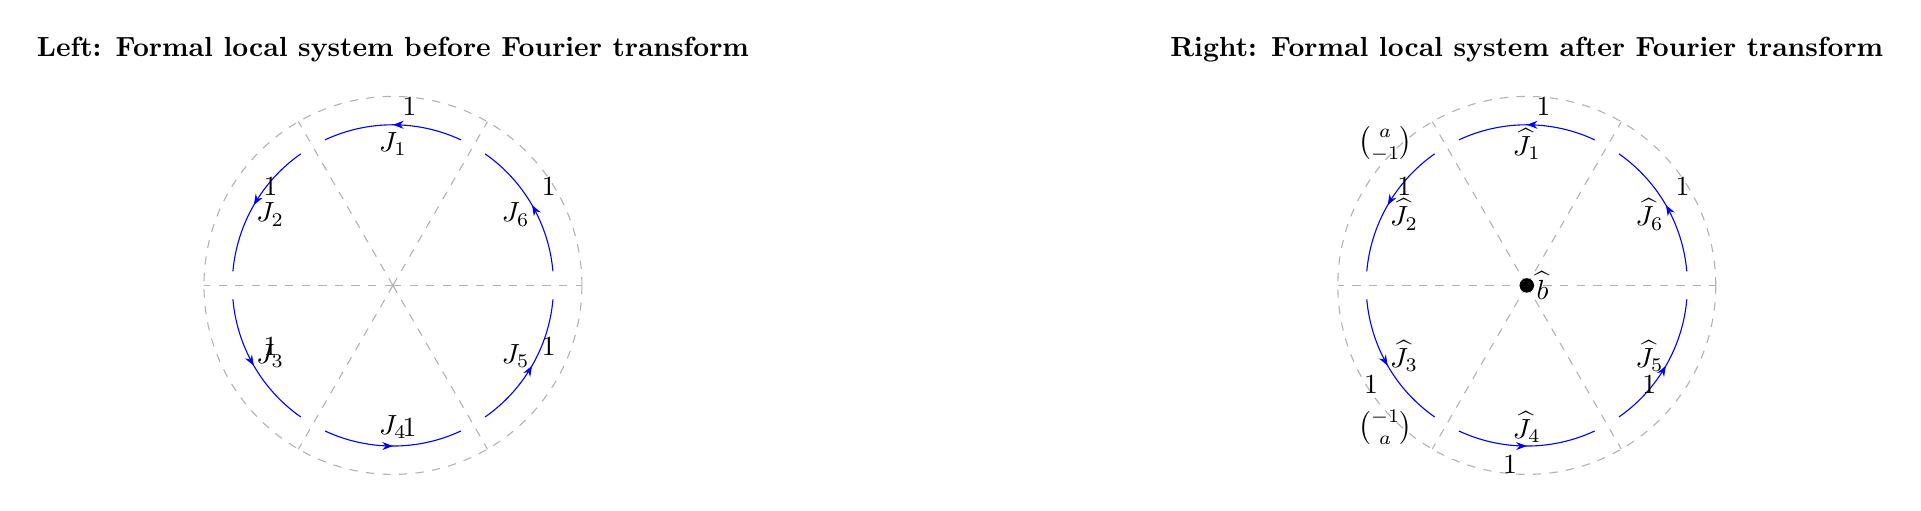
\begin{tikzpicture}[scale=1.2]

% Draw the left diagram: Formal local system before Fourier transform
\begin{scope}[shift={(-6,0)}]
    % Circles and sectors
    \draw[dashed line] (0,0) circle (2);
    \foreach \i in {1,...,6} {
        \draw[dashed line] (0,0) -- ({\i*60}:2);
        \node at ({\i*60+30}:1.5) {$J_{\i}$};
    }
    
    % Arrows and labels
    \foreach \i/\j in {1/2,2/3,3/4,4/5,5/6,6/1} {
        \draw[myarrow, blue] ({(\i-1)*60+5}:1.7) arc ({(\i-1)*60+5}:{\i*60-5}:1.7)
            node[midway, above right, black] {$1$};
    }
\end{scope}

% Draw the right diagram: Formal local system after Fourier transform
\begin{scope}[shift={(6,0)}]
    % Circles and sectors
    \draw[dashed line] (0,0) circle (2);
    \foreach \i in {1,...,6} {
        \draw[dashed line] (0,0) -- ({\i*60}:2);
        \node at ({\i*60+30}:1.5) {$\widehat{J}_{\i}$};
    }
    
    % Arrows and labels
    \foreach \i/\j/\k in {1/2/{\binom{a}{-1}}, 2/3/{\binom{-1}{a}}, 3/4/{\binom{a}{-1}}, 4/5/{\binom{-1}{a}}, 5/6/{\binom{a}{-1}}, 6/1/{\binom{-1}{a}}} {
        \ifnum\i<4
            \draw[myarrow, blue] ({(\i-1)*60+5}:1.7) arc ({(\i-1)*60+5}:{\i*60-5}:1.7)
                node[midway, above right, black] {$1$};
        \else
            \draw[myarrow, blue] ({(\i-1)*60+5}:1.7) arc ({(\i-1)*60+5}:{\i*60-5}:1.7)
                node[midway, below left, black] {$1$};
        \fi
    }
    
    % Base point and matrices
    \filldraw[black] (0,0) circle (2pt) node[right] {$\widehat{b}$};
    \node at (-1.5,1.5) {$\binom{a}{-1}$};
    \node at (-1.5,-1.5) {$\binom{-1}{a}$};
\end{scope}

% Add labels to indicate the diagrams
\node at (-6,2.5) {\textbf{Left: Formal local system before Fourier transform}};
\node at (6,2.5) {\textbf{Right: Formal local system after Fourier transform}};

\end{tikzpicture}
\end{document}